\documentclass[11pt]{article}
\usepackage{amsmath}
\usepackage{graphicx}
\begin{document}
\section{Analyzing the Data}

Since we are interested in the fluctuations of the mean power density, we don't care about the actual structure of the spectra's mean that we measure, except that it verifies that we are indeed in the cavity resonance by seeing the cavity structure. In general we want to remove any structure to make sure we are not weighting variations towards one end of the channel more because of some structural offset. Actually that doesn't make any sense. I give up.

What really makes sense we have fluctuations but must determine a mean somehow, and to do that we need to fit the curve. I have discussed above the equivalent circuit of the cavity or at least attempted to. The structure we observe is due to the electronics plus the response of the cavity. The reason we observe a dip in general seems to be because of the fact that the noise of the LNA is higher than the temperature of the cavity, so it acts as a source which is then reflected from the cavity input according to the reflection coefficient, which is a long winded way of saying the LNA noise from the front end is making an $S_{11}$ measurement for us.

Again, because the observed structure in the spectra is a sum of the electronics plus cavity response, figuring out the cavity response only means subtracting out the electronics structure.  Even when doing that there seems to be some asymmetry in the observed profile around the resonant frequency, which is probably due to impedance mismatches along the many connections and long waveguide lengths. 

One of the reasons we care about monitoring the cavity's resonant frequency is that we do not have an automatic way of making sure the cavity does not drift. We try to keep the temperature stable although this can vary from run to run whether the temperature flucutates by 0.1 K or 1 K. Sometimes helium gets into the cavity, which then rapidly decreases the resonance frequency. Although we can observe this from the change in the spectra once this happens (noise fluctuations increase, noise mean increases when not on resonance), it is just one other check that could be implemented.


If we had a way to switch between filters quickly that would be very nice, since for the two cavity experiment we want to reduce all unneccessary bandwidth so we usually focus on a 1 MHz passband, but then it is difficultt to make sure the cavity has not drifted while taking the measurement. We could also have these filters in parallel, so that one measurement is of a wideband to monitor the cavity and the other is of the short bandwidth to acquire data quickly and average it.

Although I have presented the noise from the LNA as a good thing, initially we tried to get rid of it because it makes the modeling more difficult (having to account for noise waves impinging on the cavity that may or may not be spectrally flat) and also because for frequencies $f \neq f_0$ that are still within the cavity response, the noise waves at that frequency will partially reflect from the coupling hole and then be transmitted back to the LNA, increasing the noise. Not sure if this is the correct picture. In fact not sure if this is experimentally seen, that the width of the curve increases in the sloped bits.

\section{Noise Modelling}
\subsection{Cavity Equivalent Circuit}
PUT IN PICTURE OF EQUIVALENT CIRCUIT
\begin{figure}
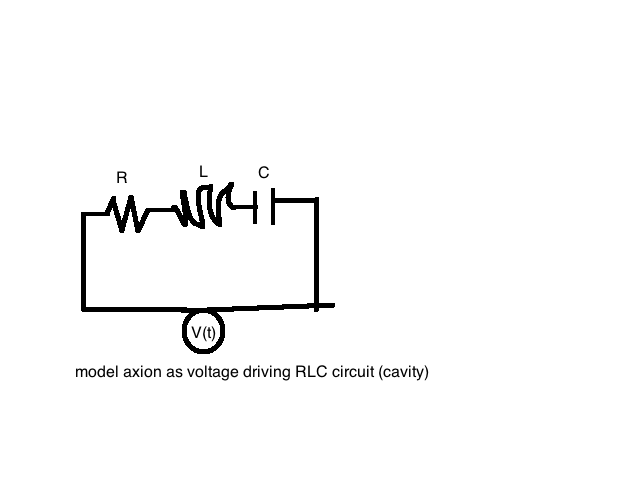
\includegraphics[scale=0.8]{RLCcircuit}
\end{figure}

\begin{figure}
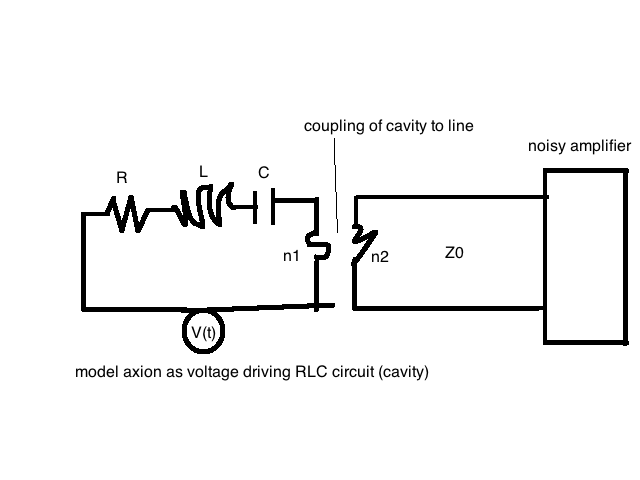
\includegraphics[scale=0.8]{RLCcircuitNoisyAmplifier}
\end{figure} 

The equivalent circuit of a 3D cavity is an RLC circuit. Whether it is in series or in parallel does not matter - the values of the components will change in order to keep the same Q, but the general phenomena - a resonant frequency with damping characterized by some value, is all that is important.
Let us take a series RLC circuit. One such circuit that has a Q of 8000 and a resonant frequency of 34.29 GHz has R = 50 ohms, L  1.62e-9 H and C = 1.32e-15 F. If we add the strong coupling hole, we can model it as a mutual inductance with $n=\frac{1}{1-\beta}$ where $\beta$ is the coupling coefficient that relates the unloaded Q to the loaded Q: $\frac{\beta}{1+\beta}Q_u = Q_l$. $\beta$ is measured by doing a reflection measurement and taking $|S_{11}(\omega_0)| =$ check this.

\subsection{Wave Model of Two-Port Noise}
Reference the Meys paper and Haus.

Here we will explain how we got the model that we used.

We can compare it to the ADMX model.

\section{Noise}

The background we are limited by are the fluctuations in thermal radiation. The variations are random, so we can model it as Gaussian so that the variations reduces as $1/\sqrt{N}$, where N is the number of averages. The fluctuations of the energy density in the range $\omega, \omega +d\omega$ vary as $kT$ so reducing the temperature reduces the fluctuations. Bandwidth is an important consideration - by reducing the spectrum of frequencies we capture, we can speed up our acquisition time, but we have a lower limit on our bandwidth placed by the constraint that anywhere the cavity resonates could potentially produce a signal (this is for the axion case). Therefore we must at least take in a spectrum with width $\delta f = f/Q$. As well, we need to be able to resolve structures on the scale of the expected axion bandwidth, which is expected to be some number based on considerations of velocity dispersion in the Earth. So we must have $\delta f/f_a$ channels, or bins, or $f_a$ must be our maximum resolution bandwidth. I say maximum, when I mean to say optimum.

Although we said above that the fluctuations go down as the number of averages, what that means in terms of the bandwidths we discussed above is that for a total time of data acquisitiong $t$, the resolution bandwidth will be $1/t$, which we want to make equal to $f_a$. If we average over all m bins, where $m=\delta f/f_a$, then $m =\delta f t$. This makes no sense.

The fluctuation in a given channel will go down as the square root of the number of measurements made that are averaged together. If there are $N$ measurements constituting a total time $t=Nt_m$, where the time of each measurement gives a resolution bandwidth by the uncertainty principle of $t_m=1/f_a$, then $t=N/f_a$ and $N=tf_a$. So the fluctuation in our channel will go down as $1/\sqrt{t f_a}$. This is known as the Dicke radiometer equation and was put forward to clarify issues in reducing noise for radioastronomy, where people where looking at noise-like traces and trying to reduce their fluctuation. Although here we are limited to a maximum bandwidth of $f_a$ if we want to resolve our axion-bandwidth, in general for reducing noise, a larger bandwidth is desirable to reduce the variations more quickly.

For the two cavity experiments where we expect to see a signal at exactly one frequency, I'm actually not clear on why at the moment, the structure will have a very small bandwidth and so our resolution bandwidth will be accordingly small.

The signal to noise ratio is the ratio of the expected signal power over the noise fluctuation amplitude squared. If we write this in terms of power densities, then if the signal power is in a bandwidth $f_a$ with power density $\rho_a$

This is $\frac{\rho_0}{kT/(f_a\sqrt{N})} = \frac{\rho_0}{kT}\sqrt{\frac{t}{f_a}} $.

Lowering the temperature increases the signal to noise ratio. Models are made predicting smaller $f_a$ which would also increase the signal to noise ratio.

The temperature is given by the physical thermal temperature of the cavity plus the effective temperature of the LNAs, which add noise due to electron scattering in the transistor and loss. The noise, referenced to the input of the LNAs, can be represented in terms of a thermal temperature $T_e$. The noise temperature $T_e$ of the first LNA is approximately 15 K when cold (cold means 4 K).

We are in the process of doing a noise temperature measurement to determine this $T_e$ exactly.


\section{Splitting into I and Q}

Why do we split into I and Q? No reason, as far as I can tell. For the axion experiment, there really is no reason since we do not expect some phase relationship...
For the two cavity experiment as well. We implement phase locking, whatever that means, so isn't that enough?
Anyways can't change it now.

\section{Sensitivity}
The SNR is given as
$$\text{SNR} = \frac{P_{\text{sig}}}{P_{\text{noise}}}$$

where $$P_{\text{noise}} = \sigma_T\times resBW = \frac{k_B T_{\text{sys}}}{\sqrt{resBW \cdot \tau}}\times resBW$$

and the expected power from the axion is $$P_{\text{sig}}=(gB_0)^2 C V Q_l \rho_a/m_a$$
spread out over a bandwith $$B_a = m_a/Q_a$$

where the axion quality factor (determined  by the velocity dispersion) is $$Q_a = 10^6$$
so for an axion mass of $$m_a = 34\text{ GHz ,}$$
the axion bandwidth is
$$B_a = 34\text{ kHz .}$$
Going back to the sensitivity equation, we have the following values for the $\text{TM}_{020}$ mode:

$$B_0 = 7\text{ Tesla} = 7\text{ T}\times195.35\text{ eV}^2/1\text{ T} = 1367.45 \text{ eV}^2$$
$$C_{020} = 0.13$$
$$V = 1.6 \text{ cm}^3$$
$$Q_l = 10^4$$
$$\rho_a = 0.3\times10^9 \text{ eV}/\text{cm}^3$$
$$m_a = 1.4 \times 10^{-4} eV $$

which gives a value of $$P_{\text{sig}} = (8.3\times10^{21} \text{eV}^4) g^2.$$

The noise power is determined by the resolution bandwidth and the noise temperature: if we set
 $$T_{\text{sys}} = T_{\text{noise}} + T_{\text{cav}} = 15 + 5 = 20\text{ K}$$
and 

$$resBW = B_a = 34 \text{ kHz}$$

then using the fact that 
$$k_B = 8.617\times10^{-5}\text{ eV/K}$$ 
and 
$$1 s = 1.519 \times 10^{15} \text{ eV}^{-1}$$ 
we get
 $$P_{\text{noise}} =  \sqrt{2.2\times10^{-11}\text{ eV}} \times 0.00172 \text{ eV} \times \frac{1}{\sqrt{\tau}} = 8.08\times10^{-9}\text{ eV}^{3/2} \frac{1}{\sqrt{\tau}}$$

so in order to get a signal to noise ratio of 5 
$$SNR = 5$$

and a coupling slightly better than the CAST limit of
 $$g = 0.6 \times 10^{-10} 1/GeV = 0.6 \times 10^{-19} 1/eV$$

we need an integration time of 
\begin{multline}
$$\tau = (SNR^2 \times (8.08\times10^{-9})^2 \text{ eV}^3) /P_{\text{sig}}^2= (1.63\times10^{-15} \text{ eV}^3)/(3\times10^{-17}\text{ eV})^2 \\ = 1.81 \times 10^{18} eV^{-1} = 1195\text{ sec} =20\text{ min}$$
\end{multline}
and if we want to get a factor of two below the CAST limit, meaning a coupling of

$$g = 0.4 \times 10^{-10} 1/GeV$$

then the integration time must be

$$\tau = 45\text{ min}$$

\section{Bin Edge or Scalloping Loss}

We have neglected to include the possibility that the axion will not be in the center of a frequency bin. Due to the nature of a discrete fourier transform, if a delta function is so far away from the center you will lose XX amount of power. 

We can write this as XX.

Therefore we must take the worst case limit where the axion is between two bins as our estimate of the power, and thus reduce the expected power by 40%.

\section{Maxwell Tail}

We must also account for the fact that the Maxwell tail is not in the same bin as the peak, so we lose 20% of the power that way.

PICTURE OF A BOOSTED MAXWELLIAN



\section{Data Acquisition Time}
The NI-USB 5132 digitizer has a buffer size of 30 MB, can have sampling rates up to 50 MSa/sec, and has three channels (two channels for multichannel acquisition, and a third for setting an external clock, otherwise it uses the internal 50 MHz clock).

Each trigger can capture up to the buffer size of 30 MBytes of data; since each data point is an 8 bit number, if you are acquiring two channels at once, you can get 30 million data pairs from one trigger (am I a factor of two off here?).

For a sampling rate of $$F_s = 10\text{ MHz}/\text{sec}$$ you can capture $$\text{onetriggertime} = 30 \text{ Mpoints}/F_s = 3 \text{ sec}$$ worth of data in one trigger.

To get the 45 minutes of data needed for the factor of two limit (see Integration Time page), you need $$45\text{ min} \times 60\text{ sec/min }/ 3 \text{ sec/trigger} = 900\text{ triggers}$$

Right now the bottleneck comes I think comes from the throughput on the USB connection. The USB cord is 2.0, so it typically takes 1 min per trigger from start to stop when actually running DigitzerDAQ. CHECK THIS...

This means  it would take 15 hours to acquire the 900 triggers worth of data, which could conceivably be done in one day, if someone takes a day shift, and someone takes a night shift. 

\section{FFT}

The Fourier Transform of the data is accomplished using the FFTW libraries which are fast fourier transfoms. We also use the ROOT software package as the host for our code. We take a complex FFT of the I and Q channels separately and then square the individual spectra and add them.

When averaging we take the power density spectra and average these. There is some trickiness to averaging the linear scale and then converting to logarithmic or taking the average of logarithmic traces. I can't remember what that is.


\subsection{Minuit}

MINUIT is a code that can fit fifth order polynomials according to Michael Hotz. Do they need initial parameters? I don't know.

The noise wave model can also be done using a current and voltage noise source. Maybe I will try this instead, don't really see the advantage or reason of doing the noise wave model.


\section{Windowing}

We use what is called a square window, which means not doing any windowing. This can lead to spurious frequencies and also depress the amplitude of your actual signal, but we don't care.
ADMX (Michael Hotz) uses square windowing.
Maybe we should use flat top windowing for the two cavity experiment. Michael Betz does.

In any case using a window means you have to integrate for longer because you lose some data so it broadens your resolution bandwidth, so to tighten it back down you have to integrate for longer.

\section{Data Analysis}

The data analysis starts from the raw time traces. The receiver chain at the final step separates the signal into an in-phase and quadrature component using an IQ mixer. These two separated signals each go through a low pass filter with approximately 4 MHz bandpass, and then are amplified by a voltage pre-amplifier with a gain of 5. The output channels (labeled henceforth as I and Q) are then plugged into a PCI 1154 card on a Dell desktop and digitized at a rate of 10 MSa/sec, with a a digital external referene at 10 MHz. We have a data acquisition program written in Visual C$\#$ that acquires however many records we desire, with each record containing 2.56e6 samples. The data acquisition has zero deadtime. The regular running procedure is to take 15,000 records at one particular cavity setting, and then retune - 15,000 records takes 1.06 hrs. 

\section{EXPECTED SENSITIVITY}

The expected sensitivity we expect to achieve assuming we are dominated by statistical effects is determined by the axion power we wish to determine. The theoretical axion power on resonance in the cavity is given by 

Psig = XXX

For the power reaching the amplifier, the power is multiplied by a coupling factor kappa = beta/(1+beta).

For usual parameters of the experiment

Clmn = xxx

Qloaded = xxx

B = xxx

V = xxx

The signal to noise ratio is SNR = Psig/Pnoise, where the fluctuations in the noise power are Pnoise and given by the radiometer equation

$Pnoise = Tsys/\sqrt{b*t} $

For a cavity temperature of 10 K and a system noise temeprature whih is the sum of the cavity physical temperature, amplifier temperature, and effective noise temperatre of the first amplifiers, we determined this by a Y-factor measurement to be 25 K. The resolution bandwidth b should be equal to the bandwidth of the axion. While there are different models for how the energy dispersion of the axion should look, the simplest model assumes that the axions are a cold almost motionless gas of particles. Their virializiation in the galaxy provides their energy dispersion - virialization meaning that the gravitational attraction from the galaxy means that in order to not escape the galaxy the axions must have a potential energy uncertainty equal to their kinetic energy SOMETHING SOMETHING.

The next simplest distribution for the axion would be to have a Maxwell-Boltzmann distribution of the energies. This can be written in terms of the energies as XXX

Turner in Periodic Signatures of the Axion or Windows on the Axion Universe modifies this by including the rotation of the earth, to yield a distribution of XXX which has a Q of $10^{-6}$.

If we ignore that for now and assume that the axion is a delta function, our signal to noise ratio is determined by 

Psig/Pnoise.

With an integration time of 1 hr, we can get a SNR of XXX.

\section{DATA ANALYSIS PART 1}

Starting with the raw time traces of the I and Q channel, each 37.5 GB in length, we perform a discrete Fourier transform on each using the FFTW Software library implemented in C. The two FFTs are squared and summed to yield a periodogram - the power FFT. The reason we have the FFT on both the I and Q channel is to be able to distinguish the positive frequencies from the negative frequncies, which would be impossible if we had mixed down to DC without the I and Q separation.

Once we have the FFT, which is performed for a fixed number of points (in our case 294 - set by what we think the axion bandwidth is and our sampling rate) we then continue to perform FFTs on the time trace data and average the resulting FFTs together. There is no overlap done. There is also no window, or to rephrase, a square window on the data.

Here is a sample spectrum, which has 5e5 averages to give the output plot.

PLOT OF SAMPLE SPECTRA
\begin{figure}
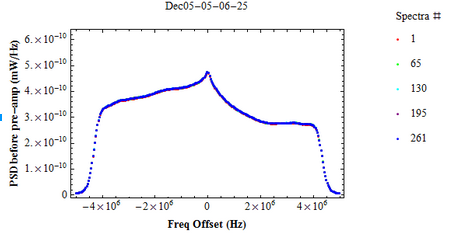
\includegraphics[scale=0.7]{samplespectrum}
\end{figure}

You can see the spike at 0 MHz which is our DC noise, the attenuation at the wings which is the result of the last 4 MHz Low-Pass filters, and the structure in the right hand side of the spectra, where the cavity is centered at 2 MHz. 

\section{THE CUTS}

We take cuts on the data by removing the first 30 and last 30 points and also the 12 points in the middle where the DC spike occurs.

For runs taken after Jan 23, there was a test tone signal offset from the cavity resonance by -3 MHz to make sure we were seeing the correct structure. For these runs, the three bins centered on the test tone signal were cut as well.

Then we are left with the following trace.

PLOT OF CUT SPECTRA WITH DIP
\begin{figure}
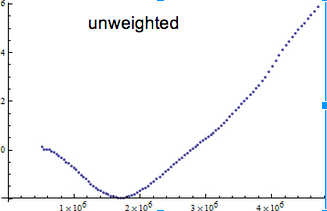
\includegraphics[scale=1]{dip}
\end{figure}

\centering 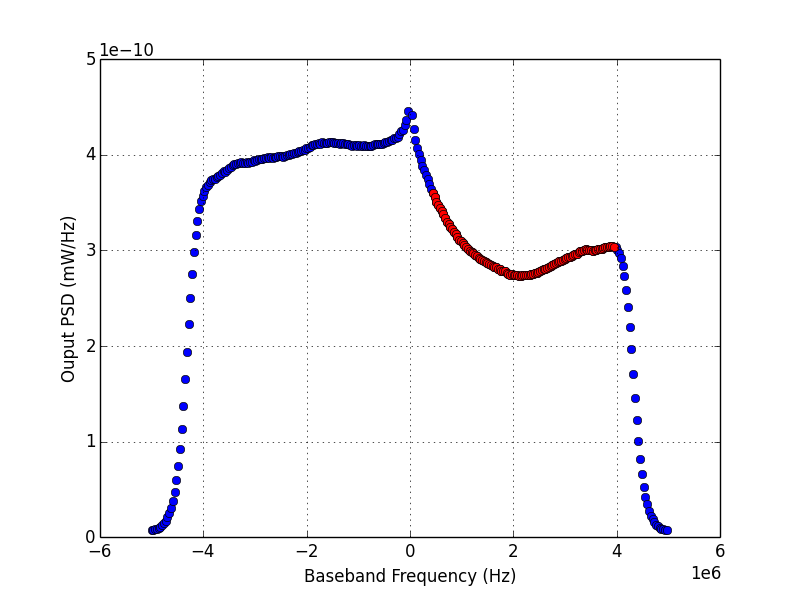
\includegraphics[width=0.6\textwidth]{cutondata}

This output spectrum has a structure due to several effects - the cavity resonance, the cavity-amplifier coupling, the waveguide, and receiver structure (dominated by the 4 MHz LPF).

\section{FITS: SMOOTHING}

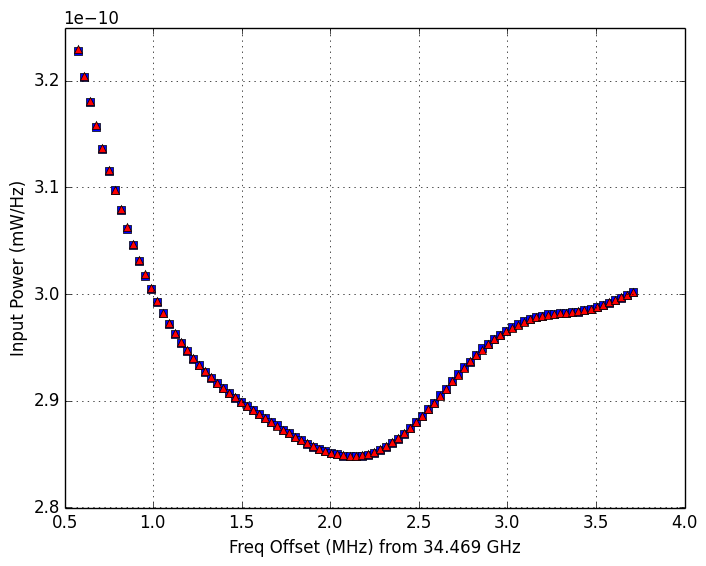
\includegraphics[width=0.3\textwidth]{Dec04-11-33-24inputpltposfreq_237}
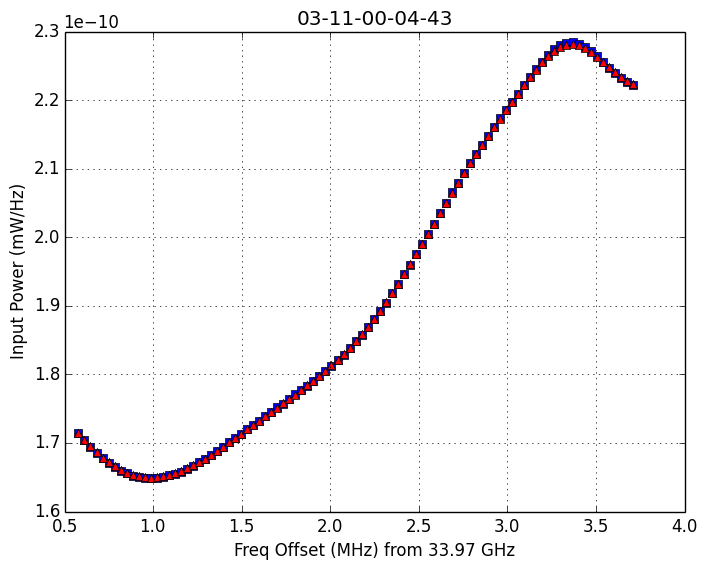
\includegraphics[width=0.3 \textwidth]{03-11-00-04-43inputpltposfreq_261}
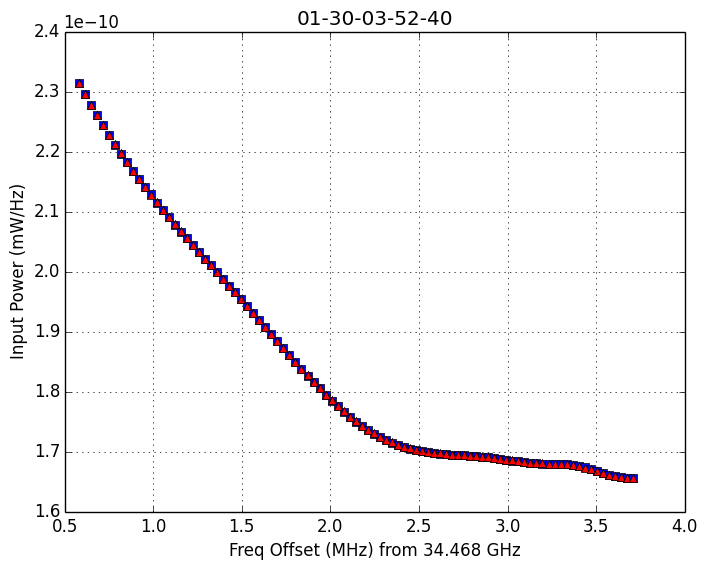
\includegraphics[width=0.3 \textwidth]{01-30-03-52-40inputpltposfreq_261}


As the receiver structure is fairly flat, we neglect its structure for now and focus on removing the cavity-amplifier structure. We can show that an equivalent circuit model of a cavity-amplifier with lossy cable in between - five free parameters - can fit the observed structure very well. We should mention that physically what is going on, broadly speaking, is that the noise from the amplifier, which is hotter than the cavity, travels to the cavity and reflects for the power spectral component that is detuned from the cavity resonance, and is absorbed for the power that is on resonance with the cavity, causing the characteristic dip you see in the spectrum above. However, there is a complicating factor caused by standing waves in the waveguide between the cavity and waveguide-coax adaptor, which causes this dip to change shape as we tune the cavity - you can see for the spectrum below, the dip is now a hump.

PLOT OF HUMP

By subtracting from the spectrum a smoothed version of the spectrum, we are able to see the fluctuations of the power about a flat background. 

PLOT OF SMOOTHED DATA
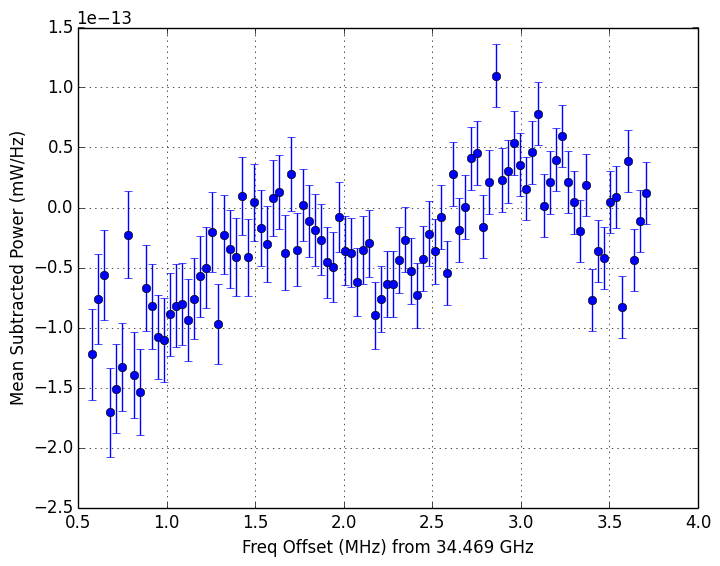
\includegraphics[width=0.3\textwidth]{Dec04-11-33-24avgsubpltposfreq_237}
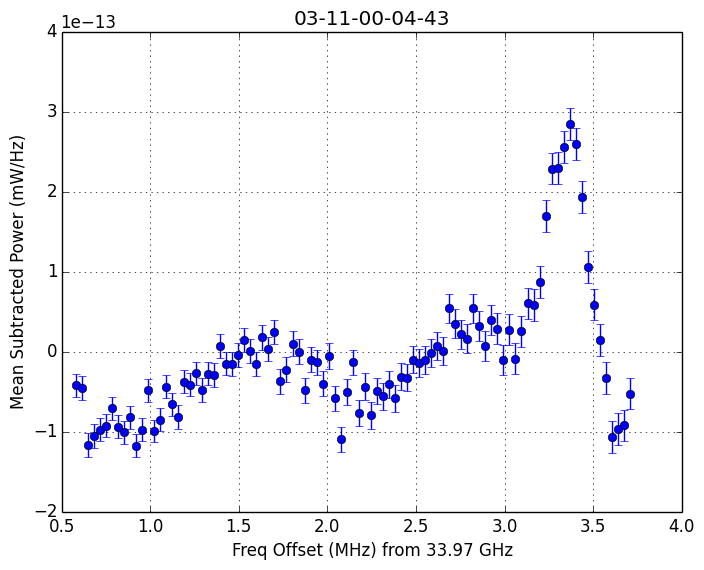
\includegraphics[width=0.3 \textwidth]{03-11-00-04-43avgsubpltposfreq_261}
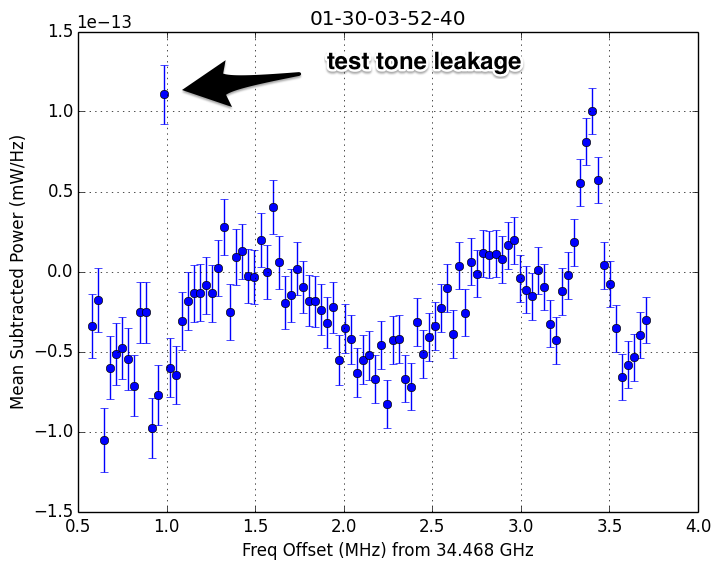
\includegraphics[width=0.3\textwidth]{01-30-03-52-40avgsubpltposfreq_261}

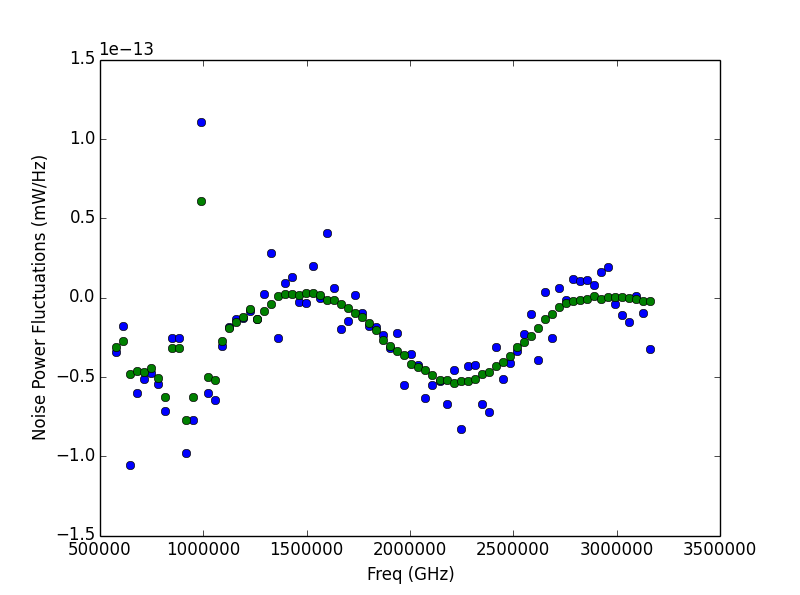
\includegraphics[width=0.29 \textwidth]{residualsub}
\includegraphics[width=0.29 \textwidth]{sub}
Secondary smoothing of residual structure

Co-adding spectra where I divide by the expected axion power for g=8.5
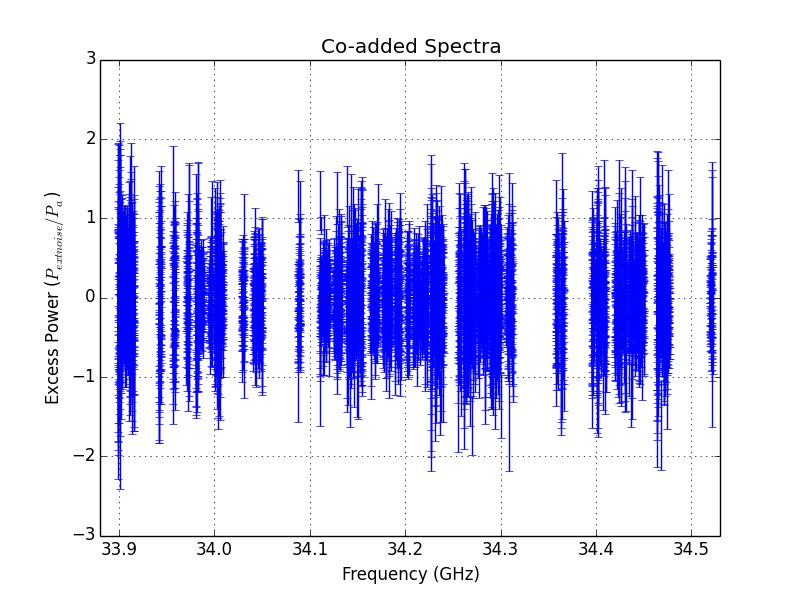
\includegraphics[width=\textwidth]{what}


By the radiometer equation, the fluctuations about the portion of the dip that are higher should have higher fluctuations, since the effective temperature is hotter. The radiometer equation predicts that for Gaussian thermal noise the fluctuations about the mean should diminish as the square root of the number of averages. What we see in practice is that the fluctuations about a flat background do indeed diminish as the square root of the number of averages. To make this plot, we averaged x spectra at a time (x=1,2...N), took a smoothed curve, subtracted it out, and then calculated the standard error of the spectrum.

PLOT of STD ERR VS NUMBER of AVGS

$P_a \sim g_{a\gamma\gamma}^2$

$P_N \sim \frac{1}{\sqrt{\tau}}$

so your exclusion bounds on $g_{a\gamma\gamma}$ go as $\tau^{-1/4}$.


\begin{tabular}{|c | c|}
\hline
$\tau$ & $g_{a\gamma\gamma}$ (1/GeV) \\ \hline
1 hr & $6\times10^{-11}$ \\ \hline
10 hrs & $3.37\times10^{-11}$ \\ \hline
20 hrs & $2.8\times10^{-11}$ \\ \hline
\end{tabular}

$\sigma$ in units of output power - translates to 12.9 K input temperature.
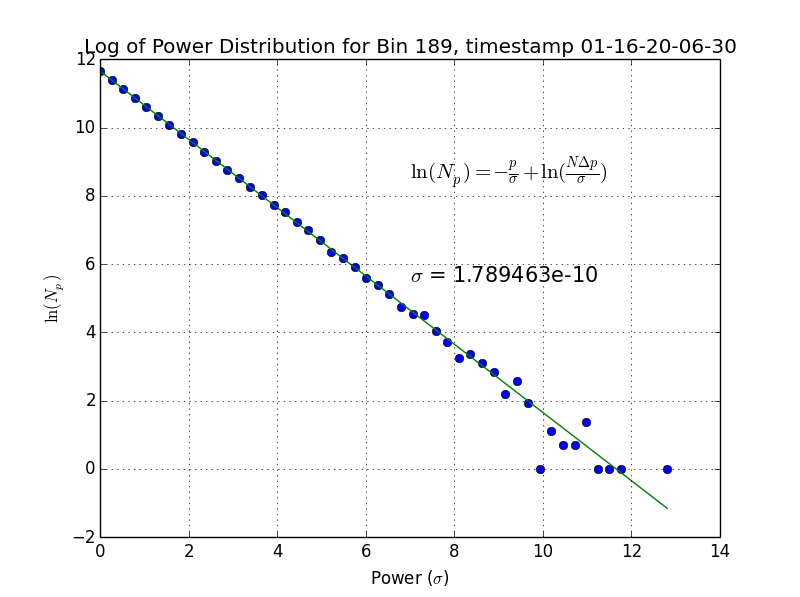
\includegraphics[width=0.8\textwidth]{logexpdistribution189}

\section{DATA STREAM}

In our data taking we stepped with stepsize 3 MHz. The bandwidth of the cavity was on average 4 MHz so there is 1 MHz of overlap between consecutive datasets. To calculate the SNR for an individual dataset, we need to know where the cavity was to calculate the expected axion power for bins detuned for the resonance, we need to know several state parameters such as the Q and form factor, and we of course need to know the noise. This will give us a SNR for an individual dataset. We then need to be able to combine the SNR’s for bins from different datasets with near identical frequencies to be able to say something about the combined dataset. SNR’s add in quadrature - we also need to make a weighted mean to get the weighted noise. The weighting factors for each bin were calculated to be $\sqrt{S/N^2}$ by Ed Daw in his thesis that maximize the noise - this is what we use here as well.

So we take the data in for each FFT saved to file, which is actually the average of 5e5 spectra, and assign a skeleton array to hold in column 1 all the frequencies that were covered in our runs, in column 2 all the power values (if there is not already a power value there), in column 3 the noise (initially set to the standard error of the spectrum), in column 4, the $weight=1/std.err^2$, in coulumn 5 the factor by which the axion power is suppressed off resonance $h[x] = 1/(1+4Delta^2/Gamma^2)$, and in column 6 the expected axion power Pi, and in column 7 the resultant SNR. If there is already a dataset value assigned to a particular frequency bin, when a new dataset is processed we combine the datasets by doing the weighted means, setting column 3 equal to.
%
\section{Runs}

\begin{table}[ht]
\caption{Summary of Runs}

\begin{tabular}{c c c c c c c c c}
\hline\hline
Run & Dates & \#Runs & \#Freqs & StableRuns & newDAQ & SwitchforRx? & SwitchforVNA? & TestTone \\ [0.5ex]
\hline
1 & Nov19-22 & x & y & z & no & some & no & no \\
2 & Dec03-07 & x & y & z & yes & no & no & no \\
3 & Dec09-13 & x & y & z & yes & no & no & no \\
4 & Dec16-20 & x & y & z & yes & some & no & no \\
5 & Jan03-05 & x & y & z & yes & yes & no & no\\
6 & Jan07-10 & x & y & z & yes & yes & no & no \\
7 & Jan23 & x & y & z & yes & yes & no & no \\
8 & Jan28-Feb1 & x & y & z & yes & yes & no & yes \\
9 & Feb04-07 & x & y & z & yes & yes & yes & yes \\
10 & Feb11-14 & x y & z & yes & yes & yes & yes \\ [1ex]
\hline
\end{tabular}
\label{table:runsummary}
\end{table}

FREQUENCY COVERAGE
\begin{figure}
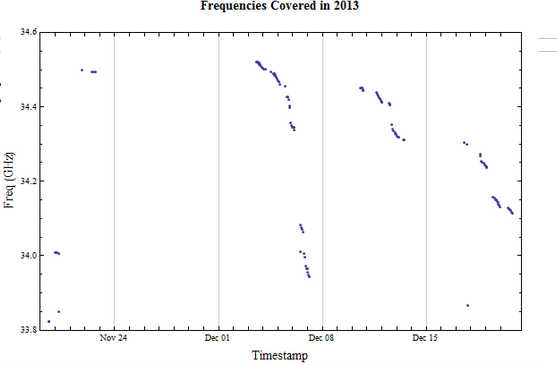
\includegraphics[scale=0.7]{frequencycoverage}
\end{figure}

OUR FINAL RESULT: EXCLUSION LIMIT PLOT

\section{Wilkinson Divider}

Wilkinson dividers or  power combiners are reciprocal devices that combine field amplitudes in phase. Although I am not interested in this property it is nice.

Using multiple cavities at the same time was tried by Darren Kinion - he used cavities tuned to the same resonant frequency and then combined the output in phase in a Wilkinson combiner. This seems hard to do for higher frequencies because the worry is that any difference in the length of the connecting parts for the two cavities would introduce a phase difference, destroying the coherent sum. 

I would propose using two different cavities at the same time that are detuned from each other. Their outputs could then have different relative phases. Although this would degrade the signal to noise ratio of each individual patch because the sum of the noise from one trace would add $\sqrt{2}$ more noise to the other patch, you would have twice as much bandwidth for looking for axions so the scanning rate is improved. Check that it is $\sqrt{2}$ not a factor of 2 degradation. Also the physical combiner is not perfect so there is some loss there. Of course you have to account for the extra time needed to analyze the traces. However, this seems less expensive than the time it takes to cool down and manually tune the cavities. One could also imagine the cavities being both tuned via a vertical insertion dielectric rod. If the rods are shifted in relative starting position, this would provide the relative detuning of the cavities.

Using multiple cavities without replicating all of the electronics (mixing scheme, LNAs, network analyzer), tuning schemes, and cryostats is the main challenge. If we take our present cryostat, the space constraint is quite tight - only two wr28 flanges can really fit.

The wilkinson divider allows one to use the same LNAs and electronics (just the mixing scheme). However as mentioned above, only two waveguides will really fit. If you have one waveguide dedicated to the LNA branch, so this is the signal coming out of the cryostat, then you only have waveguide left that can put power in. So either you give up the input waveguide altogether and rely on the LNAs to give you the $S_{11}$ measurement or use cables to couple power in and out.
\end{document}